\section{Results}

\subsection{Duration}

% \begin{figure*}[t]
%  \begin{center}
%   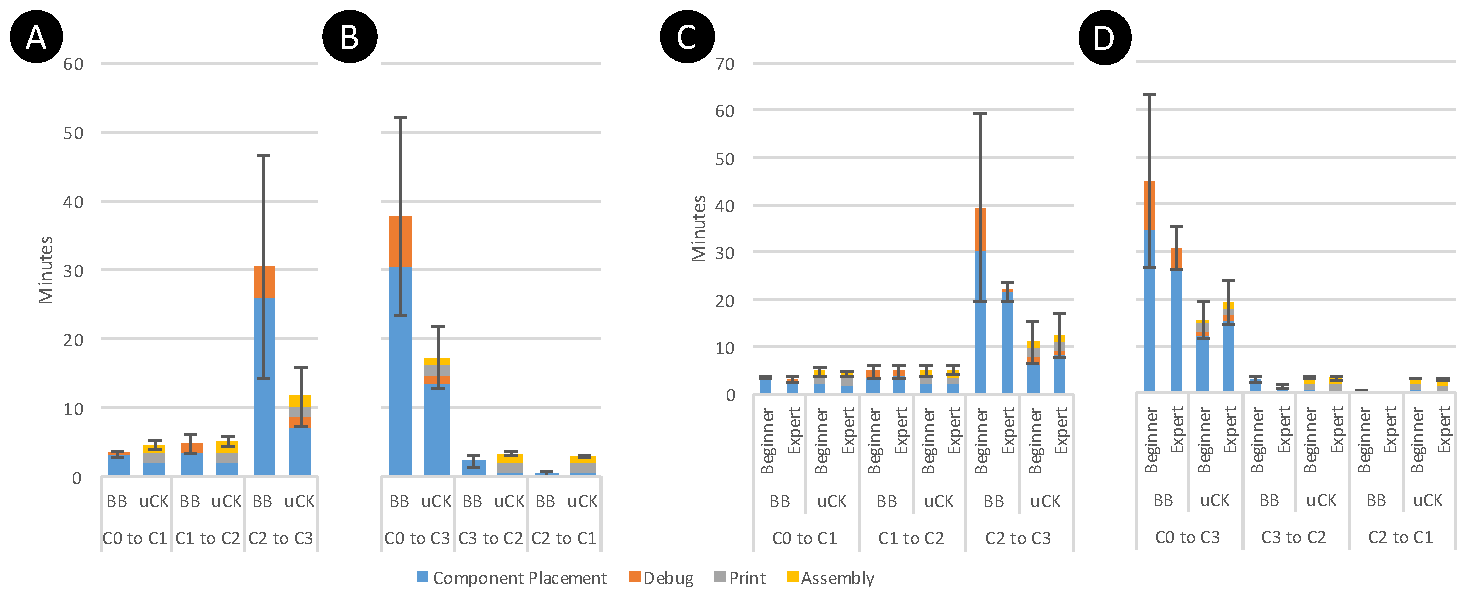
\includegraphics[width=2\columnwidth]{figures/Circuit_Construction_Duration_v10.pdf}
%   \caption{ In the following figures C1 is short for Circuit 1 and so forth. C0 means the empty scratch state. BB stands for breadboard and uCK is brief for \papertitle\. (A) Average completion time in additive sequence regardless of background. (B) Average completion time in subtractive sequence regardless of background. (C) Average completion time in additive sequence divided into beginner and expert. (D) Average completion time in subtractive sequence divided into beginner and expert. }
%   \label{fig:Circuit_Construction_Duration}
%   \end{center}
% \end{figure*}

\begin{figure}
  \begin{center}
  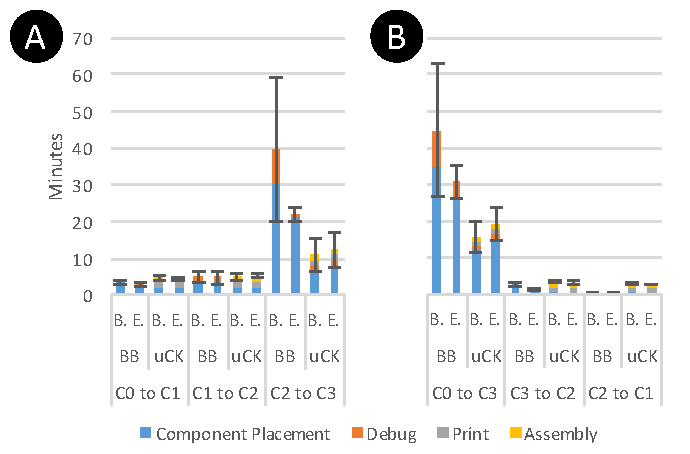
\includegraphics[width=1\columnwidth]{figures/Circuit_Construction_Duration_v14.pdf}
  \caption{In the following figures C1 is short for Circuit 1 and so forth. C0 means the empty scratch state. BB stands for breadboard and uCK is brief for \papertitle. (A) Average completion time in additive sequence divided into beginner and expert. (B) Average completion time in subtractive sequence divided into beginner and expert.}
  \label{fig:Circuit_Construction_Duration}
  \end{center}
\end{figure}

\autoref{fig:Circuit_Construction_Duration} indicates the average time durations under different circuit constructions. Comparing only the total work time of the 2 tools, neglecting user background and the sequence of circuit construction, \papertitle\ saves time up to 43\% on average  (22.4 mins vs 39.5 mins) with significant difference ($F_{0.05} (1, 30) = 18.45, p = 0.0002$).

% In an additive circuit construction sequence, regardless of user background, no significant differences were found at the transitions of \textit{Scratch to Circuit 1}  ($F_{0.05} (1, 14) = 0.98, p = 0.339$) and \textit{Circuit 1 to Circuit 2} ($p = 0.068$) between the tools. Both tools are nearly efficient under simple circuit projects. \textit{Circuit 2 to Circuit 3} has a jump in difficulty level where \papertitle\ is significant with less completion time (21.1 mins vs 38.5 mins) ($p = 0.0037$).

Regardless of circuit construction sequence and user background, \papertitle\ is slightly inefficient under simple circuits (e.g. \textit{Circuit 1} and \textit{Circuit 2}) due to printing and assembly overhead. Despite this flaw, \papertitle\ is superior under complicated circuits (e.g. \textit{Circuit 3}). \papertitle\ takes less completion time under \textit{Circuit 2 to Circuit 3} (21.1 mins vs 38.5 mins) and under \textit{Scratch to Circuit 3} (23.7 mins vs 40.5 mins), both with significant differences ($F_{0.05} (1, 14) = 0.98, p = 0.0037$, and $F_{0.05} (1, 14) = 17.25, p = 9.75 \times 10^{-4}$, respectively).

% Transition \textit{Scratch to Circuit 3} in a subtractive circuit construction sequence also shows significant difference ($p = 0.00097$) due to its high level of difficulty. However, \papertitle\ becomes inefficient at transition \textit{Circuit 3 to Circuit 2} (1.9 mins vs 2.2 mins) ($p = 0.452$) and \textit{Circuit 2 to Circuit 1} (1.5 mins vs 0.4 mins) ($p = 6.02 \times 10^{-8}$)

Since the construction time of \textit{Circuit 1} and \textit{Circuit 2} shows negligible differences between the tools, our focus is on the transitions to \textit{Circuit 3}. Building a circuit from \textit{Circuit 2 to Circuit 3}, beginner and expert average work time is 9.4 mins and 10.8 mins on \papertitle, respectively. Similar results are also presented at \textit{Scratch to Circuit 3} (15.5 mins and 19.2 mins for beginners and experts, respectively). Experts, who are familiar with breadboard's row connection pattern allowing flexible component pin placement on the same row, work slightly longer than beginners because \papertitle\ requires exact component positioning. While \papertitle\ assists both beginners and experts in building complicated circuits, \papertitle\ benefits beginners the most.

% Experts work slightly longer than beginners because \papertitle\ requires exact component positioning unlike breadboard's row connection pattern allowing flexible component pin placement on the same row.

%due to pre-printed PCP.

% picking the longest wires is the quickest without additional concerns of a wire segment reachable from one hole to another

\subsection{User Feedback and Observations}

% After constructing the 3 circuits, participants were asked to rate ``ease of use'' and ``ease of modification'' on a 5-point Likert Scale (1 means strongly disagree, 5 means strongly agree) for both a breadboard and \papertitle. The degree of ``ease of use'' evaluates . ``Ease of modification'' evaluates XXX.

% All of the participants rated an average of 3 ($sd = 1.15$) and 3.125 on a 5-point Likert Scale (1 means strongly disagree, 5 means strongly agree) for ease of use and modification on a breadboard, respectively.
11 of the participants reported that a breadboard becomes difficult to place or remove a component, hard to trace the connections, and troublesome to debug due to a clutter of jumper wires. Despite a range of different lengths of 22 AWG solid core wires provided 
% for mitigating the mess caused by jumper wires
, both beginners and experts tended not to use the solid core wires because the terminals of a jumper wire are easier for plugging onto a breadboard. 
% 使用者不想要用單心線來減少杜邦跳線亂象原因:
% 1. 廖敏勝:單心線太硬、杜邦線軟
% 2. 吳德彥:杜邦線比較好插,比較不會因為動到而跑掉會接觸不良,不過如果有長度剛好的單心線 我會選擇用單心線。但找適合長度所需要的時間都可以插好好多根杜邦線了。
% 3. 何柏融:杜邦線頭是硬的,比較好插入。要用單心線的話需要長度剛好一樣長。
% 4. 杜邦線上面有排針,比較不會彎掉,杜邦線比較軟,

12 of the participants commented that the structure of \papertitle\ hides most of the wires, which led to ease of use and modification. An expert also pointed out \papertitle\ works best with digital ICs such as multiplexers, shift registers, and similar components with complicated pin layouts.
Users pointed out that our prototype was too small in size and placing components became difficult. They recommended a more spacious layout for better component placement (e.g. resistors).
Another common feedback was that the color of female headers is too dark which led to precise placement being an issue due to indiscernible different between each row. A user suggested that an alternating black and white color scheme would be beneficial in precise component placement.


% complemented or commented? 權! 喔好
% 我再看看Likert Scale要怎麼塞進來
% 我覺得這具有點怪怪的,思考應該怎麼調整,我很會酸人家,但是自己的優點卻很難去敘述XD
% 真是困擾的問題 XD